\section{Domain Object Models Generation}
\labsec{ch04-domg}

The domain object generation feature is a vertical module that will affect both to
the CLI and API and therefore the compiler. It also has its own target users and in this
section we will explore its target users, the use cases and the possible requierements
for this feature.

\subsection{Target Users}
The different profiles of users that this feature focus on are the \textbf{Mid-technical} and \textbf{ShEx Developer}
profiles. Both of this profiles have the needed technical knowledge to use this feature. But both of them have
different use cases for the same feature as we will see in the next section.

\subsection{Use Cases}
As seen both profiles will have different use cases, we split this section in two so we can explore each one independently.

\subsubsection{Mid-technical User}
This user wants to generate / translate schemas in to domain object models, for that porpouse it wants to use the
provided CLI tool. \reffig{shex-lite-use-case-g-mid} illustrates the use case diagram for this target user and 
\reftab{shex-lite-use-case-g-mid} describes the use case.

\begin{figure}[h]
    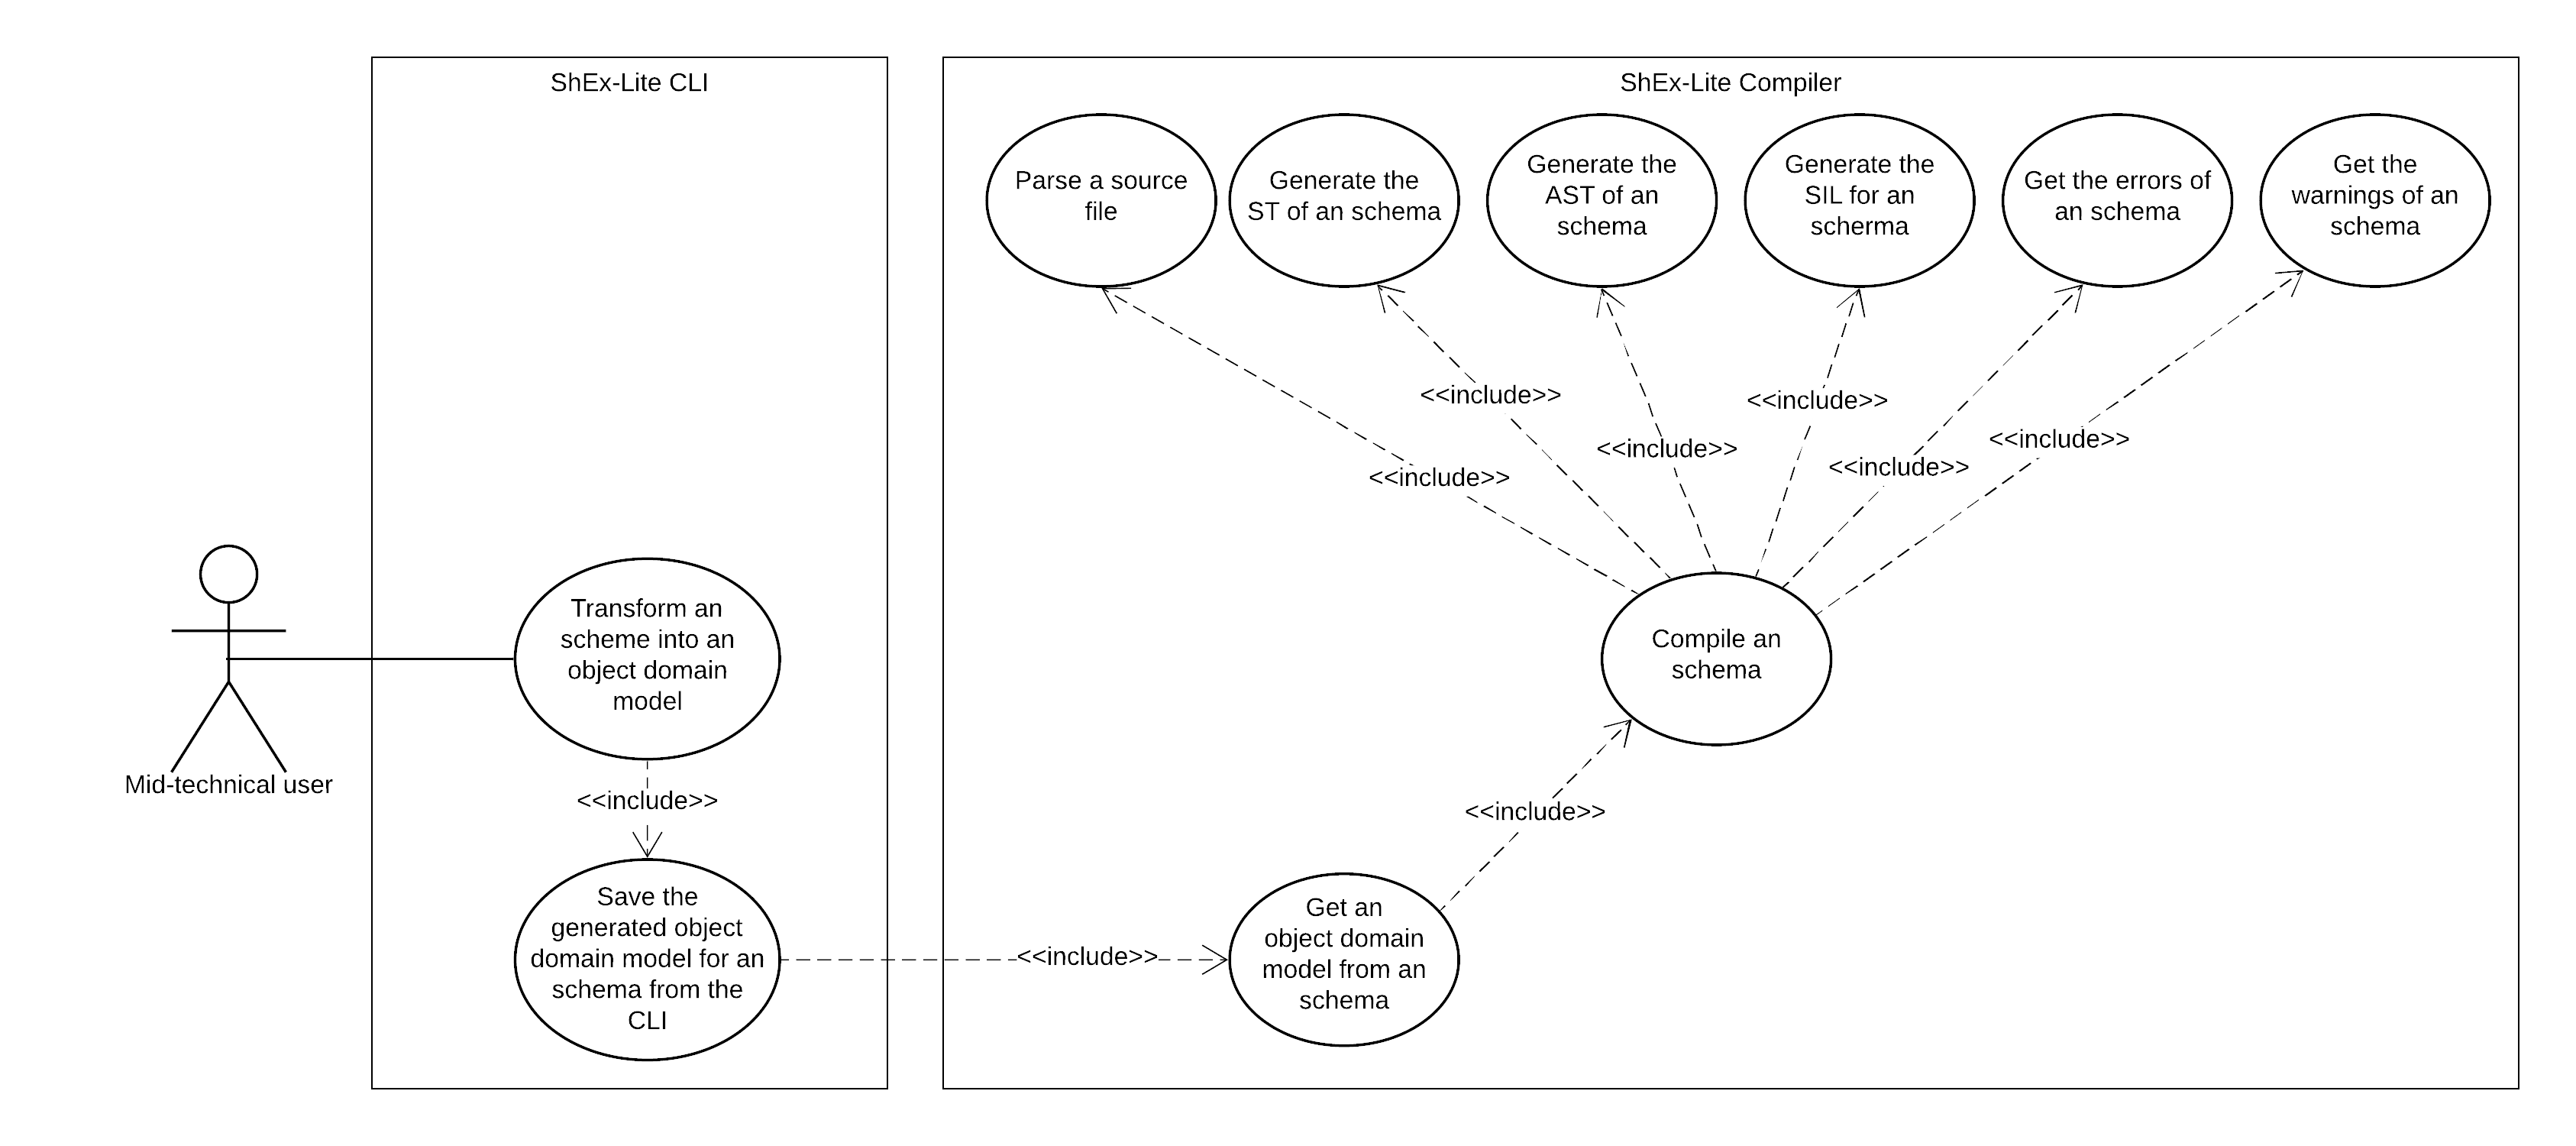
\includegraphics{shex-lite-use-case-g-mid.png}
    \caption[Domain Object Model Generation use case for mid-technical profile]{Domain Object Model Generation use case for mid-technical profile.}
    \labfig{shex-lite-use-case-g-mid}
\end{figure}

\begin{table}[h]
    \begin{tabular}{ | m{2cm} | m{8cm}| }
        \hline
        Use Case Number & 4 \\
        \hline
        Description & Generate an object domain model from an schema from the CLI tool. \\
        \hline
        Actor & Mid technical user. \\
        \hline
        Flow & The actor wants to generate an object domain model for a given schema from the CLI tool.
        For this purpose the actor introduces the schema in the CLI tool and starts the flow. Once the
        flow is complete the actor wants the generated object model to be persist as source files on his
        computer. \\
        \hline
        Conditions & For this flow to end correctly it is mandatory that the schema that the user uses to
        generate the domain object model is correct. \\
        \hline
    \end{tabular}
    \caption[Definition of the use case number 1 for the non technical user]{Definition of the use case number 
    1 for the non technical user.}
    \labtab{shex-lite-use-case-g-mid}
\end{table}

\subsubsection{ShEx Developer}
This user wants to integrate the API of the compiler in other java based applications but also wants to be able to integrate
the feature of domain object models generation in other java based applications and from the same API.

\begin{figure}[h]
    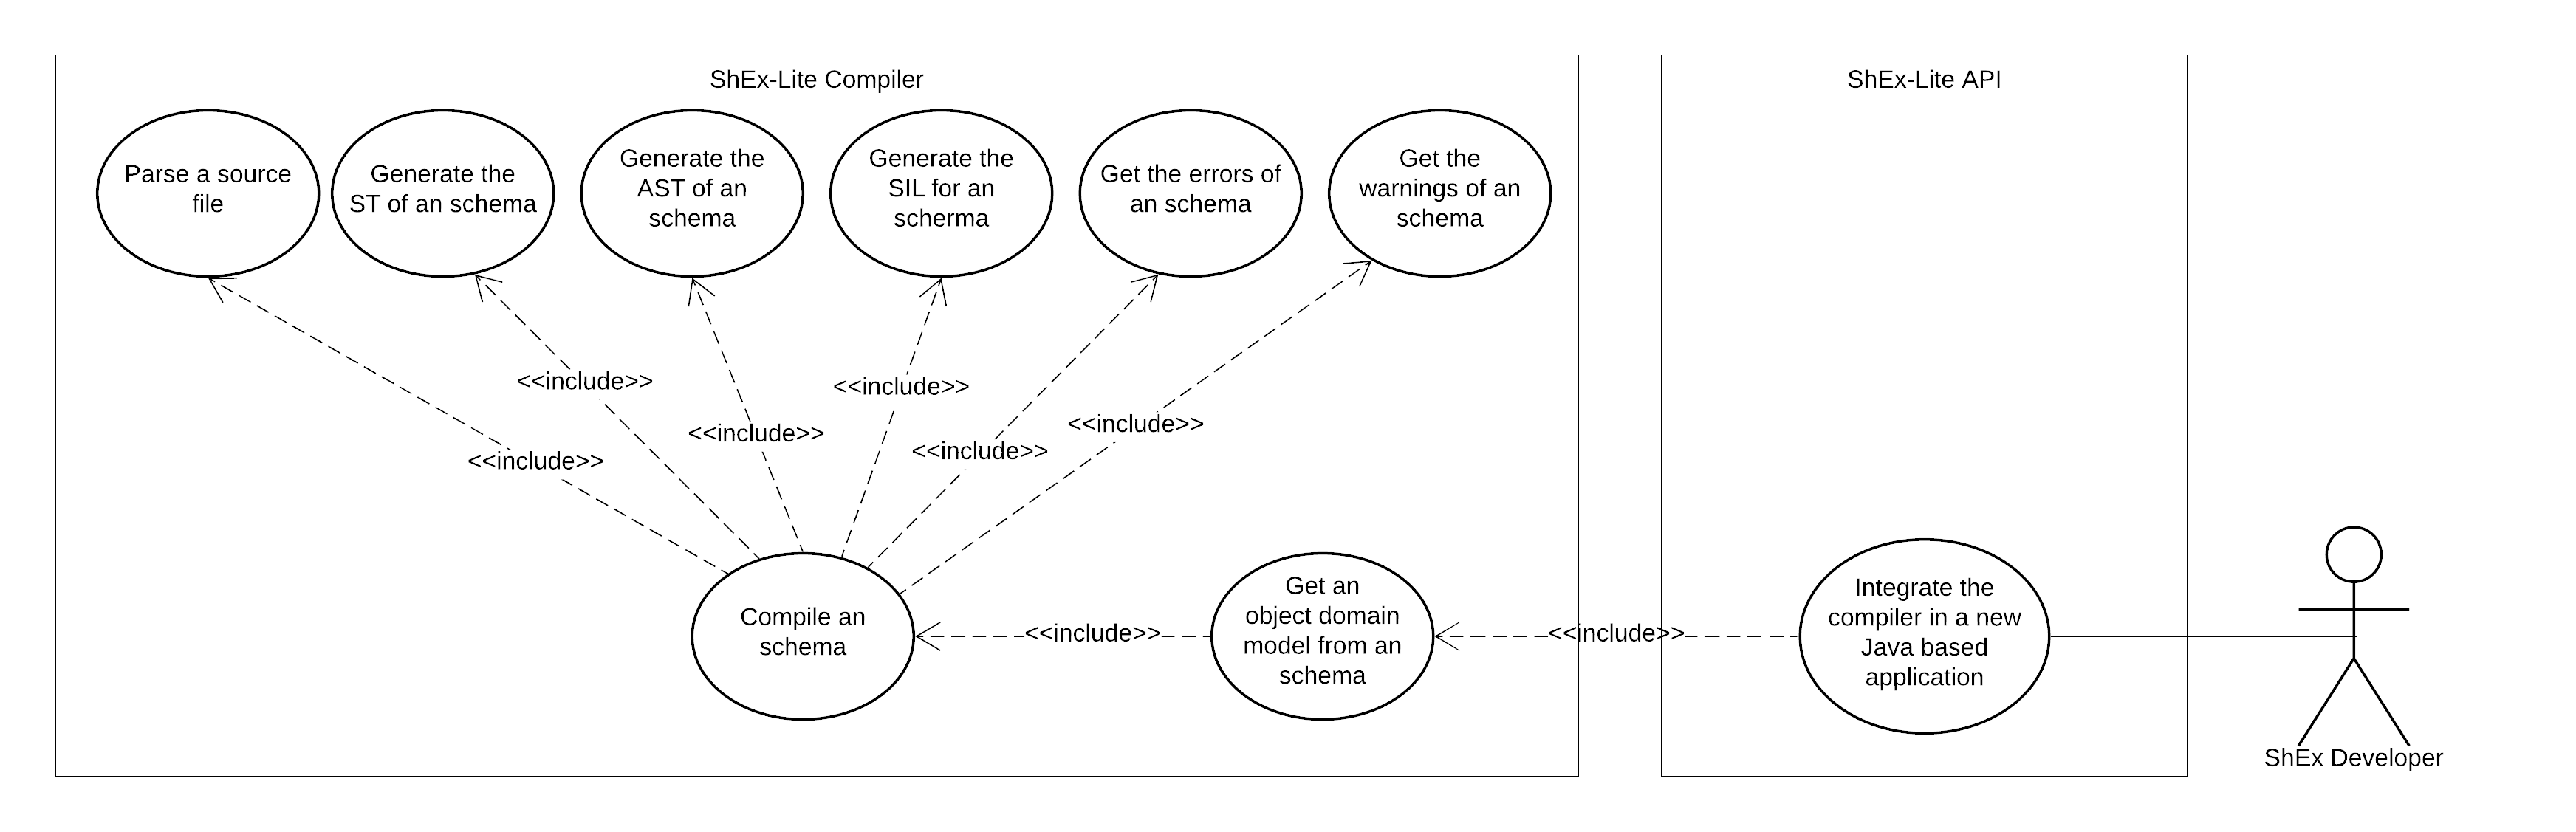
\includegraphics{shex-lite-use-case-g-dev.png}
    \caption[Domain Object Model Generation use case for mid-technical profile]{Domain Object Model Generation use case for mid-technical profile.}
    \labfig{shex-lite-use-case-g-mid}
\end{figure}

\begin{table}[h]
    \begin{tabular}{ | m{2cm} | m{8cm}| }
        \hline
        Use Case Number & 5 \\
        \hline
        Description & Integrate the generation of domain models of the API in other Java based applications. \\
        \hline
        Actor & Mid technical user. \\
        \hline
        Flow & The actor wants to integrate the generation of object domain models for a given schema from the API. \\
        \hline
        Conditions & For this flow to end correctly it is mandatory that the schema that the user uses to
        generate the domain object model is correct. \\
        \hline
    \end{tabular}
    \caption[Definition of the use case number 1 for the non technical user]{Definition of the use case number 
    1 for the non technical user.}
    \labtab{shex-lite-use-case-g-dev}
\end{table}

\subsection{Requirements}